\documentclass[12pt, a4paper]{article}

\renewcommand{\baselinestretch}{1.5}
\pagenumbering{arabic}
\pagestyle{plain}

\usepackage[margin=2cm]{geometry}
\usepackage{longtable}
\usepackage{polski}
\usepackage[utf8]{inputenc}
\usepackage{indentfirst}
\usepackage[fleqn]{amsmath}
\usepackage{graphicx}
\usepackage{float}
\usepackage[tableposition=top]{caption}
\usepackage{hyperref}
\usepackage{subfig}
\graphicspath{ {./graphics/}}
\hypersetup{
    colorlinks=true,
    linkcolor=blue,
    filecolor=magenta,      
    urlcolor=blue,
    pdfpagemode=FullScreen,
    }

\newcommand\HREF[2]{\hyper@linkurl{#2}{#1}}

\author{Jakub Bożek}

\title{Sprawozdanie z PCA}
\begin{document}

\begin{titlepage}
    \centering
    {\LARGE \bfseries Sprawozdanie z PCA \par}
    \vspace{1cm}
    
    {\Large Techniki eksploracji danych wielowymiarowych \par}
    \vspace{2cm}
    
    {\LARGE \bfseries Jakub Bożek \par}
    \vspace{0.5cm}
    
    {\large 285665 \par}
    \vspace{0.5cm}
    
    {\large Bioinformatyka, II rok \par}
    \vspace{2cm}
    
    {\Large 4 czerwca 2024 \par}
    
    \newpage
    \thispagestyle{empty}

    \tableofcontents
\end{titlepage}

\section{Wprowadzenie}

    \subsection{Cel ćwiczenia}

        Celem ćwieczeń było zapoznanie się z metodą PCA(Principal Component Analysis lub po polsku analiza głównych składowych).
        Która jest jedną z metod uczenia maszynowego nienadzorowanego. 

    \subsection{Krótkie wprowadzenie do metody PCA}
        Metoda PCA polega na redukcji wymiarowości danych za pomocą przekształceń algebraicznych. Wynikiem czego będzie możliwość
        przystępniejszego zobrazowania i/lub ich analizy.
        

    \subsection{Oprogramowanie}
        Wszystkie elementy sprawozdania zostały stworzone przy pomocy języka programowania \href{https://docs.python.org/3.12/}{Python 3.12.3} z pomocą bibliotek:\\
        \href{https://numpy.org/doc/1.26/}{Numpy 1.26.4}\\
        \href{https://matplotlib.org/3.8.4/index.html}{Matplotlib 3.8.4}\\
        \href{https://pandas.pydata.org/pandas-docs/version/2.2.2/}{Pandas 2.2.2}\\
        \href{https://scikit-learn.org/1.4/index.html}{Scikit-learn 1.4.2}\\
        \href{https://seaborn.pydata.org}{Seaborn 0.13.2}

\section{Metodologia}
    \subsection{Standaryzacja danych}

        Pierwszym elementem pracy z danymi jest ich standaryzacja.
        Odbywa się to poprzez zastosowanie wzoru:
        \begin{equation}
            z_{ij} = \frac{x_{ij} - \mu_j}{\sigma_j}
        \end{equation}
        gdzie:
        \begin{align*}
            z_{ij} &= \text{zmienna ustandaryzowana}\\
            x_{ij} &= \text{zmienna niestandaryzowana}\\
            \mu_j &= \text{średnia dla obserwacji}\\
            \sigma_j &= \text{odchylenie standardowae dla obserwacji}
        \end{align*}

        Po autoskalowaniu każda zmienna posiada średnią równą 0 oraz odchylenie standardowe równe 1.
        Takie działanie sprawia, że nie bierzemy pod uwagę jednostek. Dodatkowo każda zmienna może mieć inny zakres wartości.
        W niektórych przypadkach może to wprowadzać nam błędną intuicję względem wyglądu naszych danych.

    \subsection{Macierz kowariancji}
        \def\CovX{
            \begin{bmatrix}
                Var(x_1) & \hdots & Cov(x_1, x_n)\\
                \vdots & \ddots & \vdots\\
                Cov(x_n, x_1) & \hdots & Var(x_n)
            \end{bmatrix}
        }
        
        Macierz kowariancji, jak wskazuje nazwa, jest zbiorem danych zawierającym wartości kowariancji pomiędzy
        poszczególnymi zmiennymi.

        Aby ją policzyć, stosuję się wzór:

        \begin{equation}
            Cov(X) = \CovX
        \end{equation}

        Taką macierz można przedstawić za pomocą \href{file:./graphics/cov.png}{mapy ciepła}. Wtedy można zauważyć,
        jak poszczególne zmienne korelują ze sobą.

    \subsection{Wartości i wektory własne głównych składowych}
        
        Z macierzy kowariancji należy następnie policzyć wartości i wektory własne. W tym celu skorzystałem z
        metody \href{https://numpy.org/doc/stable/reference/generated/numpy.linalg.eig.html}{eig}. Zwraca ona wartości posortowane w kolejności malejącej względem wartości własnych, nazywanymi również eigenvalues.
        Jeśli by tak nie było, należałoby samemu wykonać sortowanie w powyższy sposób. Jest to ważne, ponieważ wartości własne wyznaczają
        istotność zmiennej w zbiorze danych.

        \begin{table}
            \centering
            \caption{Zestawienie wartości własnych oraz procent wyjaśnianej wariancji przez 10 pierwszych głownych składowych}
            \begin{tabular}{lrr}
                %\toprule
                & Wartości własne & Procent wyjaśnianej wariancji \\
                %\midrule
                PC1 & 40.32 & 27.43 \\
                PC2 & 31.53 & 21.45 \\
                PC3 & 23.05 & 15.68 \\
                PC4 & 15.39 & 10.47 \\
                PC5 & 8.15 & 5.55 \\
                PC6 & 6.59 & 4.49 \\
                PC7 & 4.77 & 3.24 \\
                PC8 & 3.86 & 2.63 \\
                PC9 & 3.25 & 2.21 \\
                PC10 & 2.43 & 1.65 \\
                %\bottomrule
            \end{tabular}
        \end{table}

        \begin{figure}[H]
            \centering
            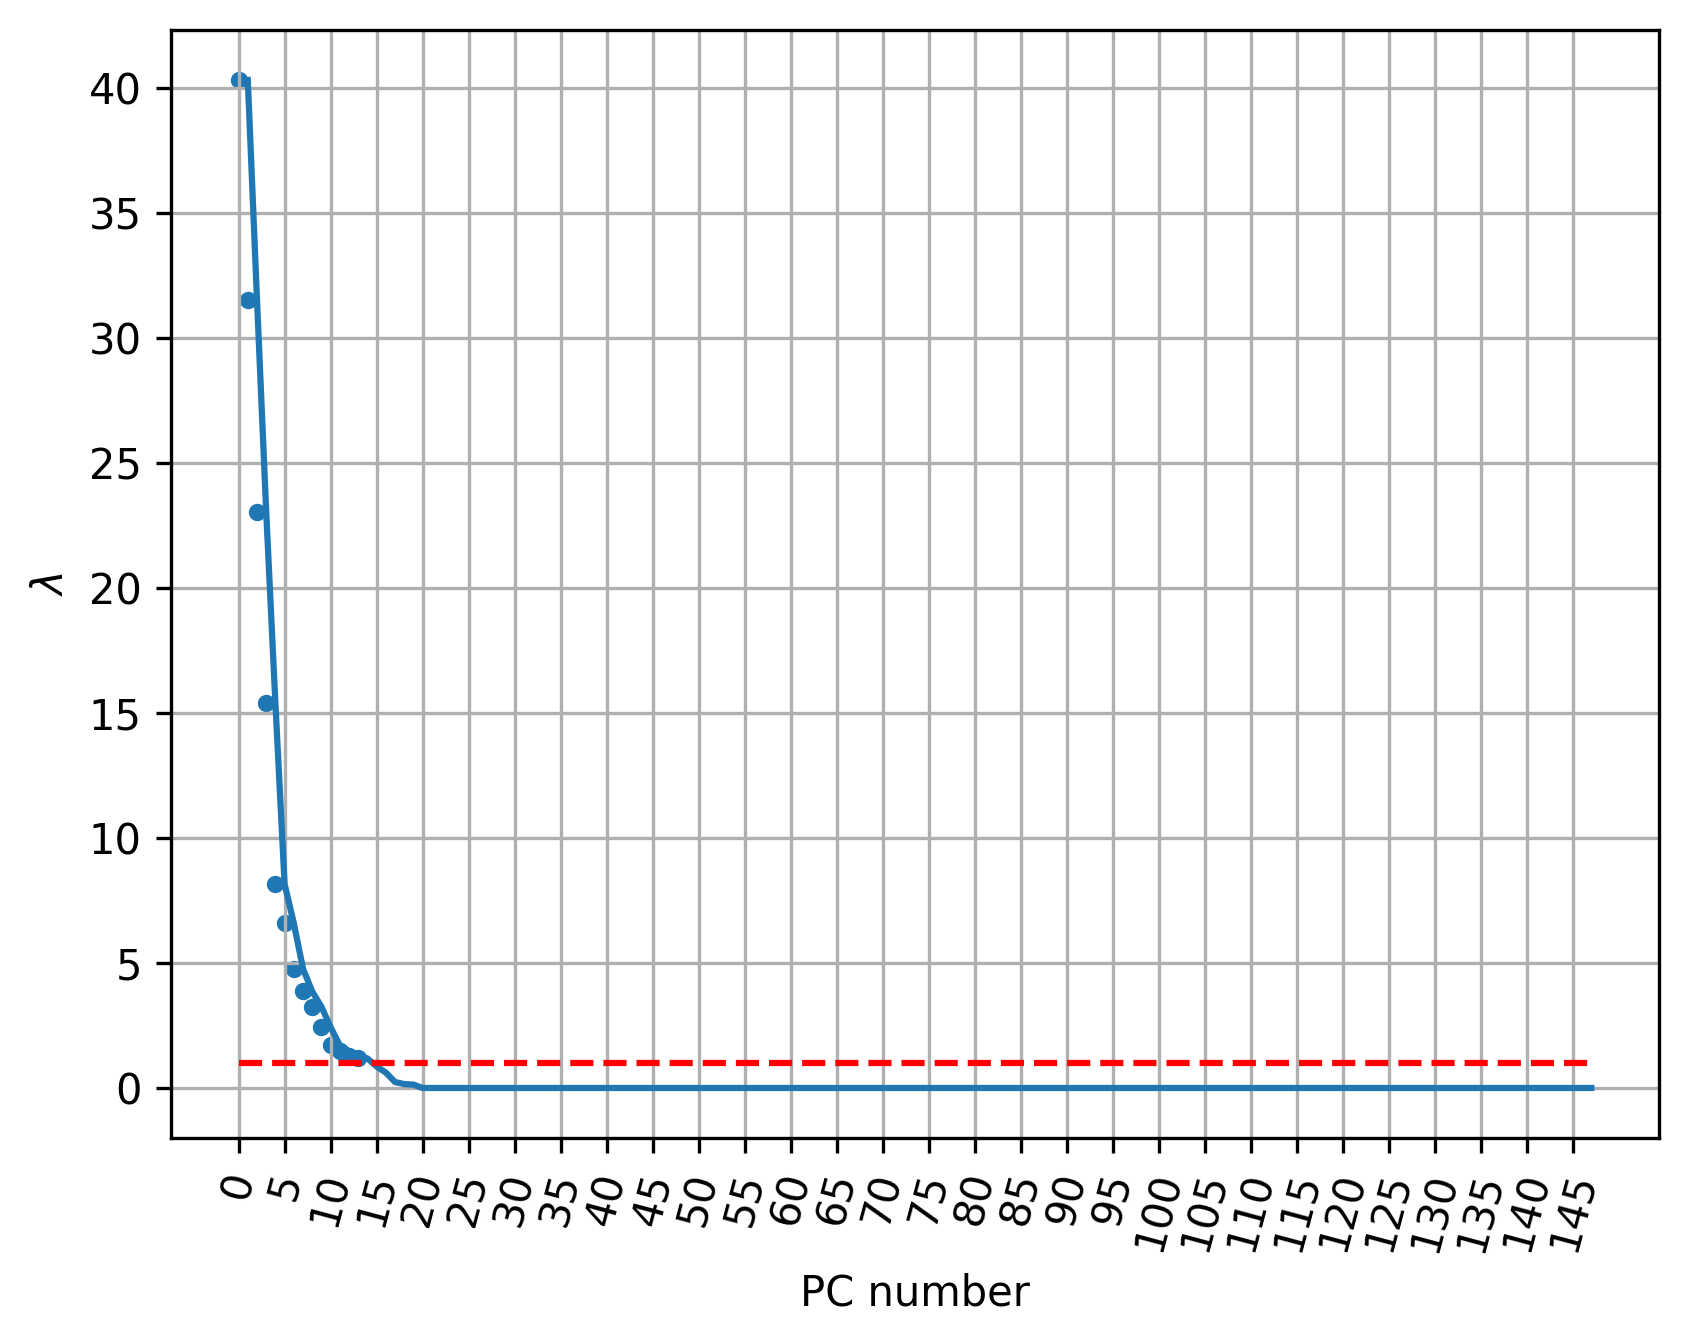
\includegraphics{eigvals.png}
            \caption{Wykres osypiska(wartości własnych) dla głównych składowych}
        \end{figure}
    
        Czerwona linia odcina główne składowe na poziomie 1. Jest to oczekiwana praktyka, jednak na potrzeby zwięzłości sprawozdania
        będę operować jedynie na 3 pierwszych głównych składowych.

        \begin{figure}[H]
            \centering
            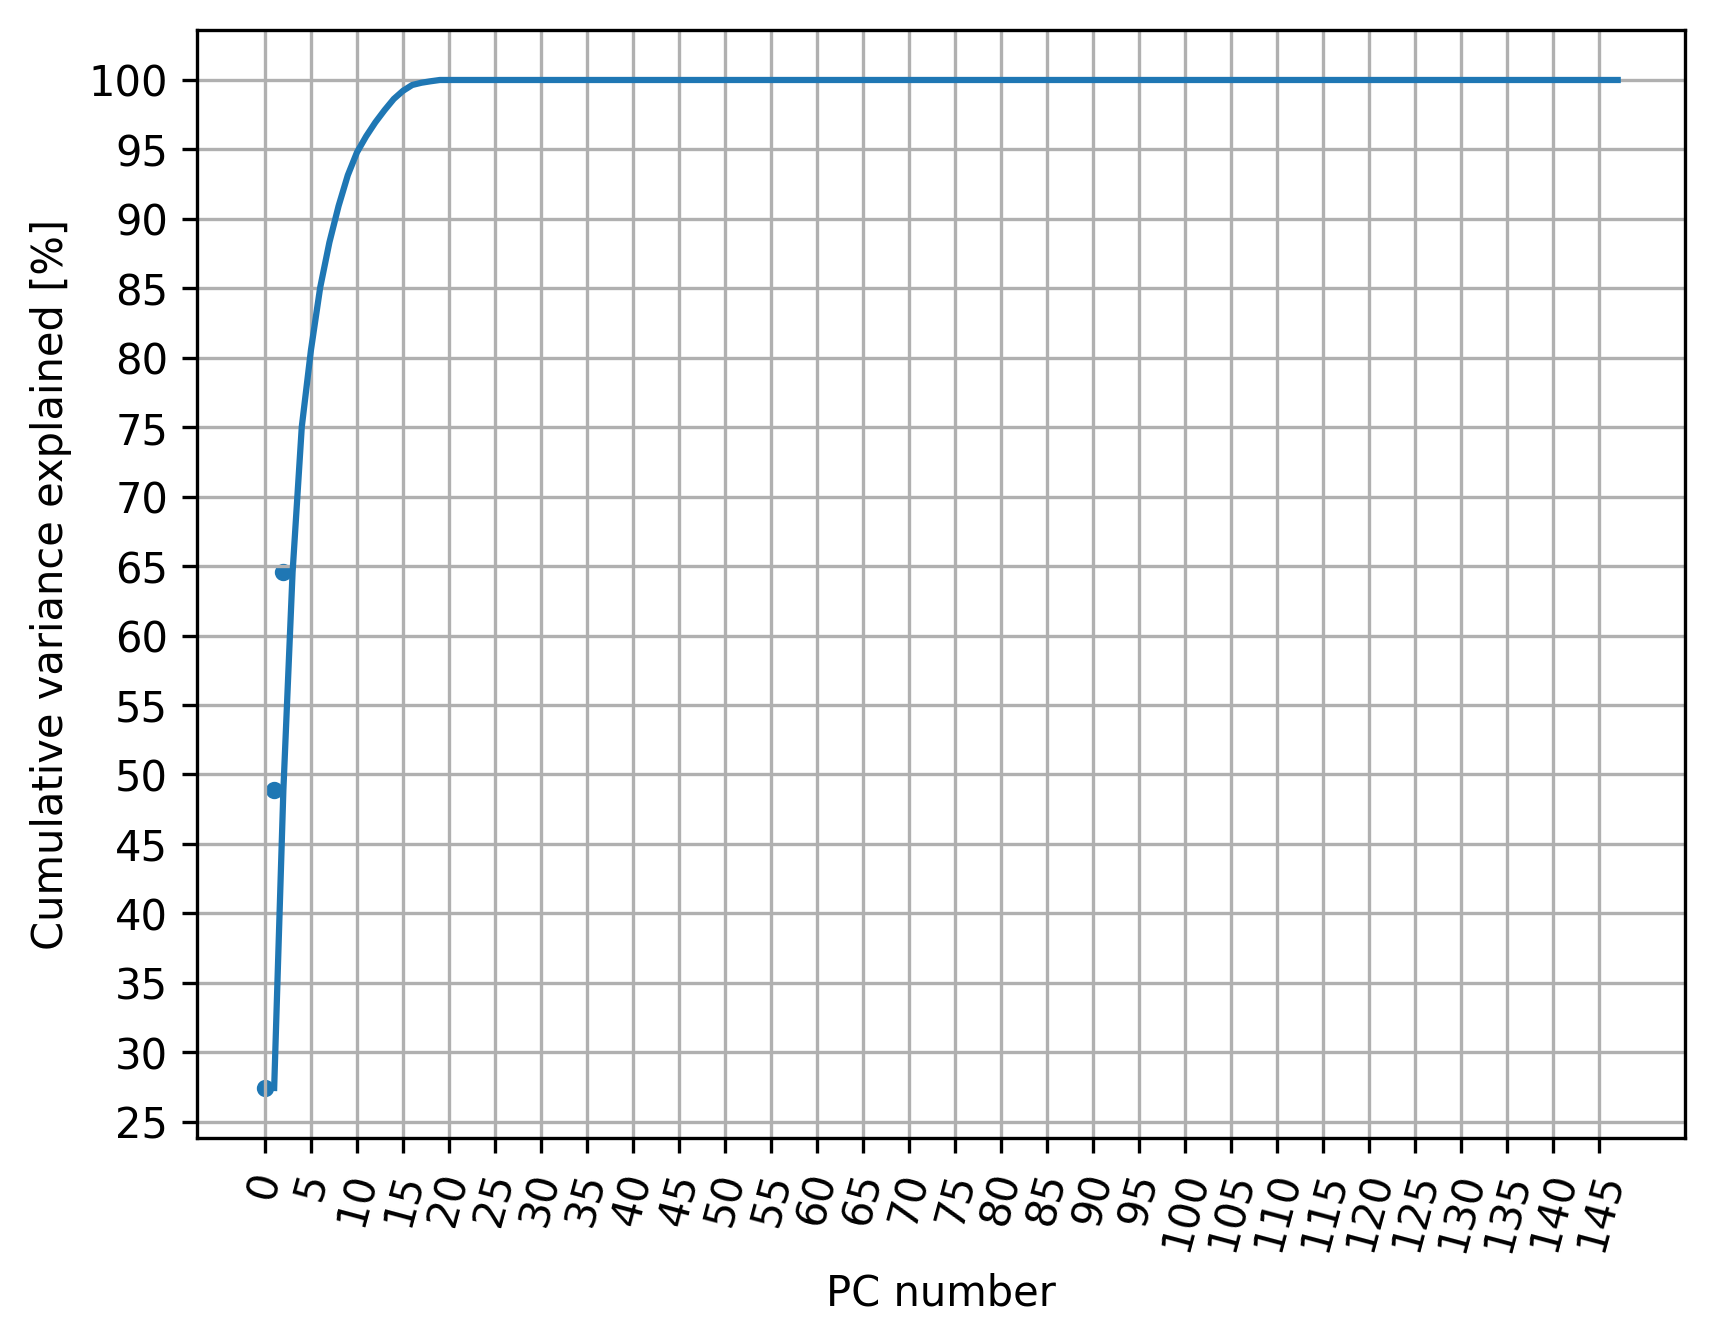
\includegraphics{cum_sum.png}
            \caption{Wykres kumulatywnego procentu wyjaśnianej wariancji przez główne składowe}
        \end{figure}

        W tym przypadku, dane będą opisywały $\sim 65\%$ wariancji całości. Normalnie byłoby to prawdopodobnie $>90\%$.
        
    \subsection{Macierz ładunków czynnikowych}
        
        \href{file:./graphics/m_lad.png}{Macierz ładunków czynnikowych} służy do przedstawienia, które zmienne mają największe znaczenie, tzn. wnoszą największą część
        informacji poszczególnym z głównych składowych. Zakłada się, że znaczenie mają te, dla których wartość bezwzględna jest większa od $0.7$.

        Aby ją policzyć, wykorzystujemy wzór:
        \begin{equation}
            M_{lad\_czyn} = \overrightarrow{v} \sqrt{\lambda}
        \end{equation}

        gdzie

        \begin{align*}
            \overrightarrow{v} &= \text{wektory własne}\\
            \lambda &= \text{wartości własne}
        \end{align*}

        \begin{table}[ht!]
            %\centering
            \caption{Typ korelacji zmiennych dla głównych składowych}
            \begin{tabular}[t]{ll}
                & PC1 \\
                MolWt & $+$ \\
                ExactMolWt & $+$ \\
                FpDensityMorgan1 & $-$ \\
                FpDensityMorgan2 & $-$ \\
                FpDensityMorgan3 & $-$ \\
                BCUT2D\_LOGPHI & $+$ \\
                Chi0n & $+$ \\
                Chi0v & $+$ \\
                Chi1n & $+$ \\
                Chi1v & $+$ \\
                Chi2v & $+$ \\
                Kappa1 & $+$ \\
                Kappa2 & $+$ \\
                PEOE\_VSA11 & $-$ \\
                PEOE\_VSA3 & $-$ \\
                PEOE\_VSA7 & $+$ \\
                SMR\_VSA3 & $-$ \\
                TPSA & $-$ \\
                EState\_VSA7 & $+$ \\
                VSA\_EState2 & $-$ \\
                VSA\_EState3 & $-$ \\
                NHOHCount & $-$ \\
                NOCount & $-$ \\
                NumAromaticHeterocycles & $-$ \\
                NumHDonors & $-$ \\
                MolLogP & $+$ \\
                MolMR & $+$ \\
                fr\_Ar\_N & $-$ \\
                fr\_pyridine & $-$ \\
            \end{tabular}
            \quad
            \begin{tabular}[t]{ll}
                & PC2 \\
                BCUT2D\_MWHI & $-$ \\
                BCUT2D\_MWLOW & $+$ \\
                BCUT2D\_MRHI & $+$ \\
                BalabanJ & $+$ \\
                BertzCT & $-$ \\
                Chi3n & $-$ \\
                Chi4n & $-$ \\
                SMR\_VSA7 & $-$ \\
                SlogP\_VSA3 & $+$ \\
                SlogP\_VSA6 & $-$ \\
                VSA\_EState1 & $+$ \\
                VSA\_EState10 & $-$ \\
                VSA\_EState6 & $-$ \\
                FractionCSP3 & $+$ \\
                NumAromaticCarbocycles & $-$ \\
                NumAromaticRings & $-$ \\
                NumHAcceptors & $+$ \\
                NumRotatableBonds & $+$ \\
                RingCount & $-$ \\
                fr\_benzene & $-$ \\
                fr\_halogen & $-$ \\ 
            \end{tabular}

        \end{table}
        %\newpage
            
        \begin{tabular}[ht!]{ll}
            & PC3 \\
            SPS & $+$ \\
            AvgIpc & $+$ \\
            PEOE\_VSA8 & $+$ \\
            SMR\_VSA4 & $+$ \\
            SlogP\_VSA4 & $+$ \\
            NumAliphaticHeterocycles & $+$ \\
            NumAliphaticRings & $+$ \\
            NumSaturatedHeterocycles & $+$ \\
            NumSaturatedRings & $+$ \\
            fr\_COO & $-$ \\
            fr\_COO2 & $-$ \\
        \end{tabular}
        
        Jeżeli korelacja jest dodatnia($+$) to wtedy wraz ze wzrostem wartości, wartość skorelowana z nią będzie również rosła.
        W przypadku korelacji ujemnej($-$) wzrost wartości oznacza spadek wartości skorelowanej.
            

    \subsection{Macierz wartości czynnikowych}
        
        Macierz wartości czynnikowych, jak możnaby uważać, powinna być liczona z poprzednio liczonej macierzy ładunków czynnikowych.
        Jednak jest to jedynie błędnie działająca intuicja, powieważ liczy się ją w sposób następujący:

        \begin{equation}
            M_{wart\_czyn} = Z \overrightarrow{v}
        \end{equation}

        gdzie

        \begin{align*}
            Z &= \text{macierz wartości autoskalowanych}\\
            \overrightarrow{v} &= \text{wektory własne}
        \end{align*}

        Przedstawia ona wartości naszego zbioru obserwacji dla każdej z wybranych głównych składowych. Te dane posłużą później do
        przedstawienia na wykresie zawierającym pary głównych składowych.

\section{Wyniki}

    Po wykonaniu kroków opisanych w poprzednim rozdziale można przedstawić wyniki na wykresach.     

    \subsection*{PC1:PC2}
        \begin{figure}[H]
            \centering
            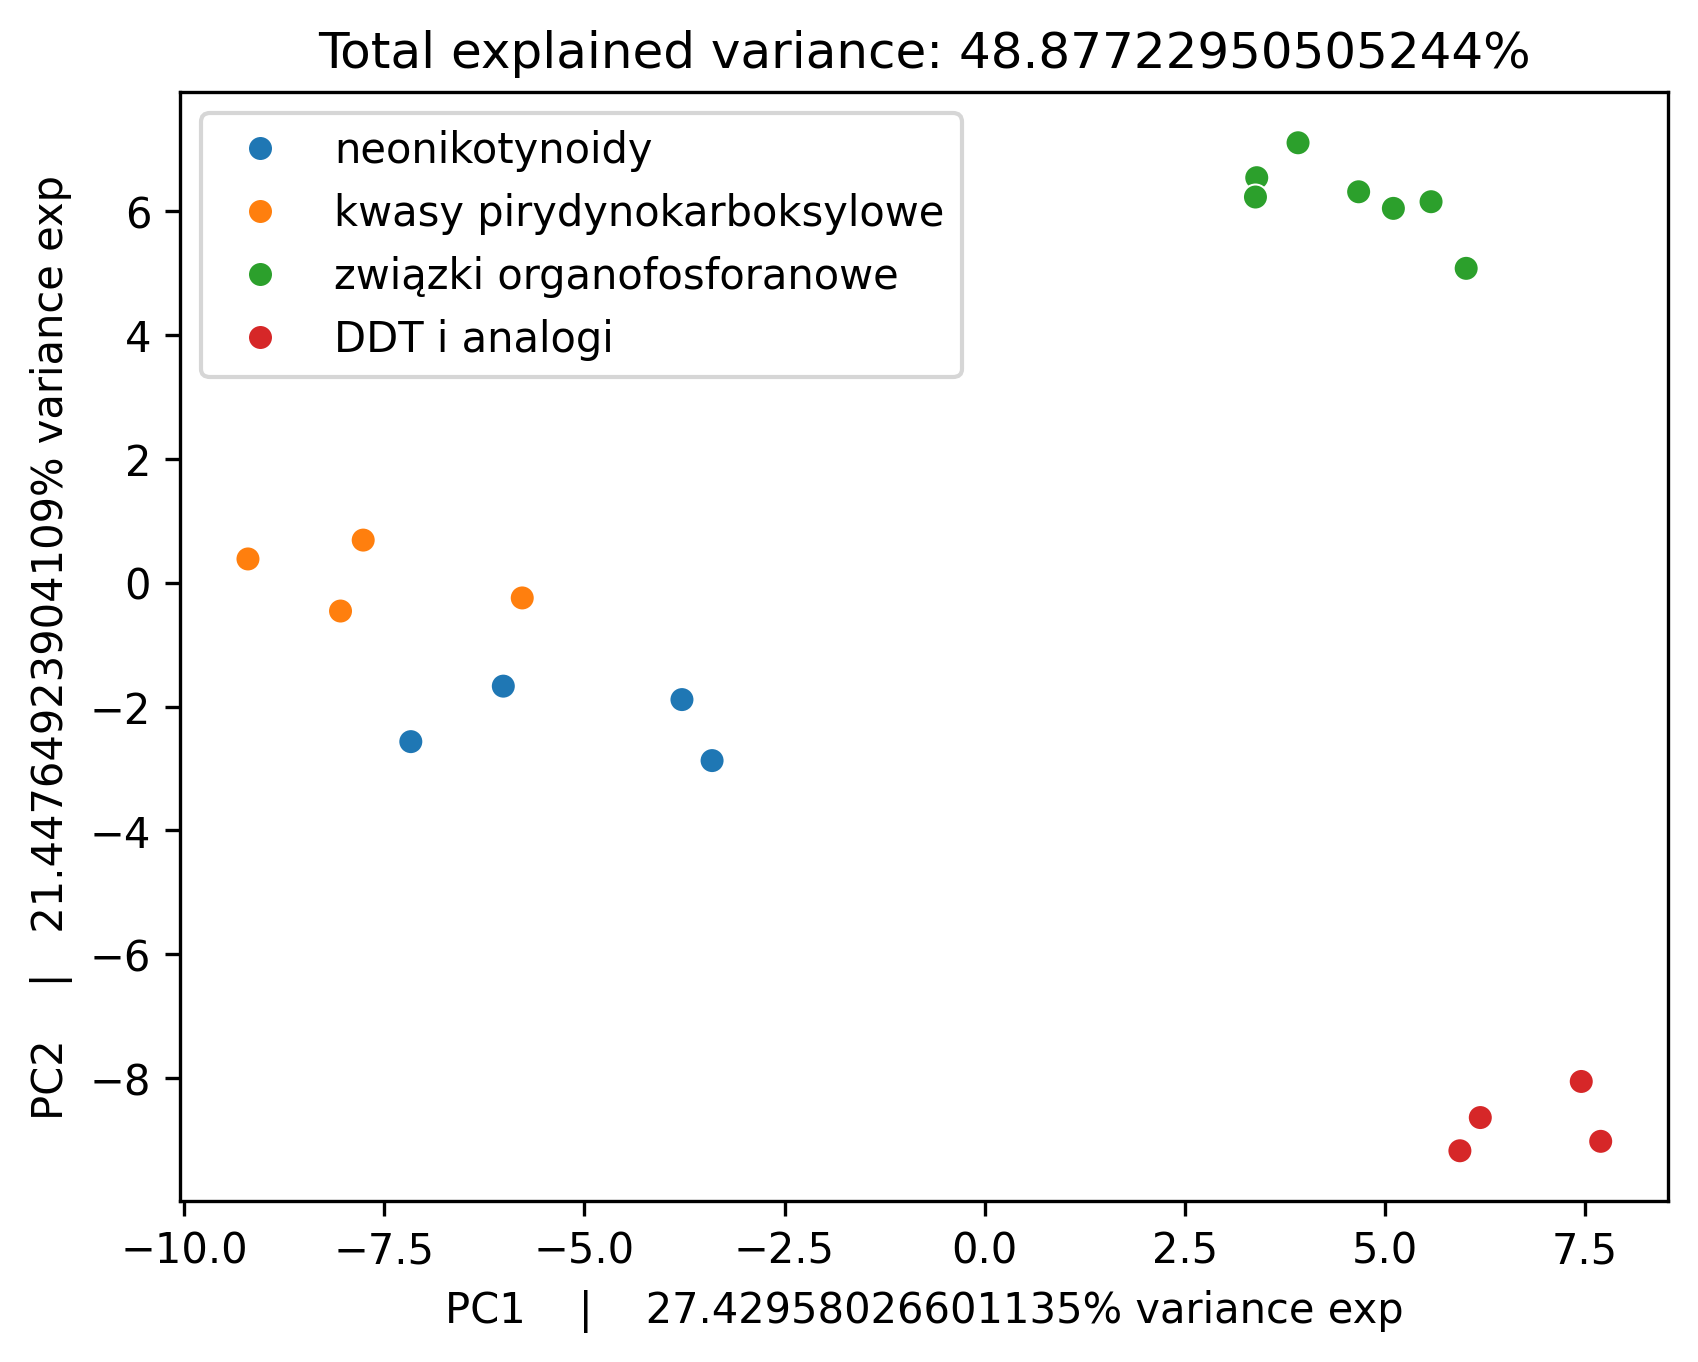
\includegraphics{12.png}
            \caption{Wykres PC1 do PC2}
        \end{figure}

    \subsection*{PC2:PC1}
        \begin{figure}[H]
            \centering
            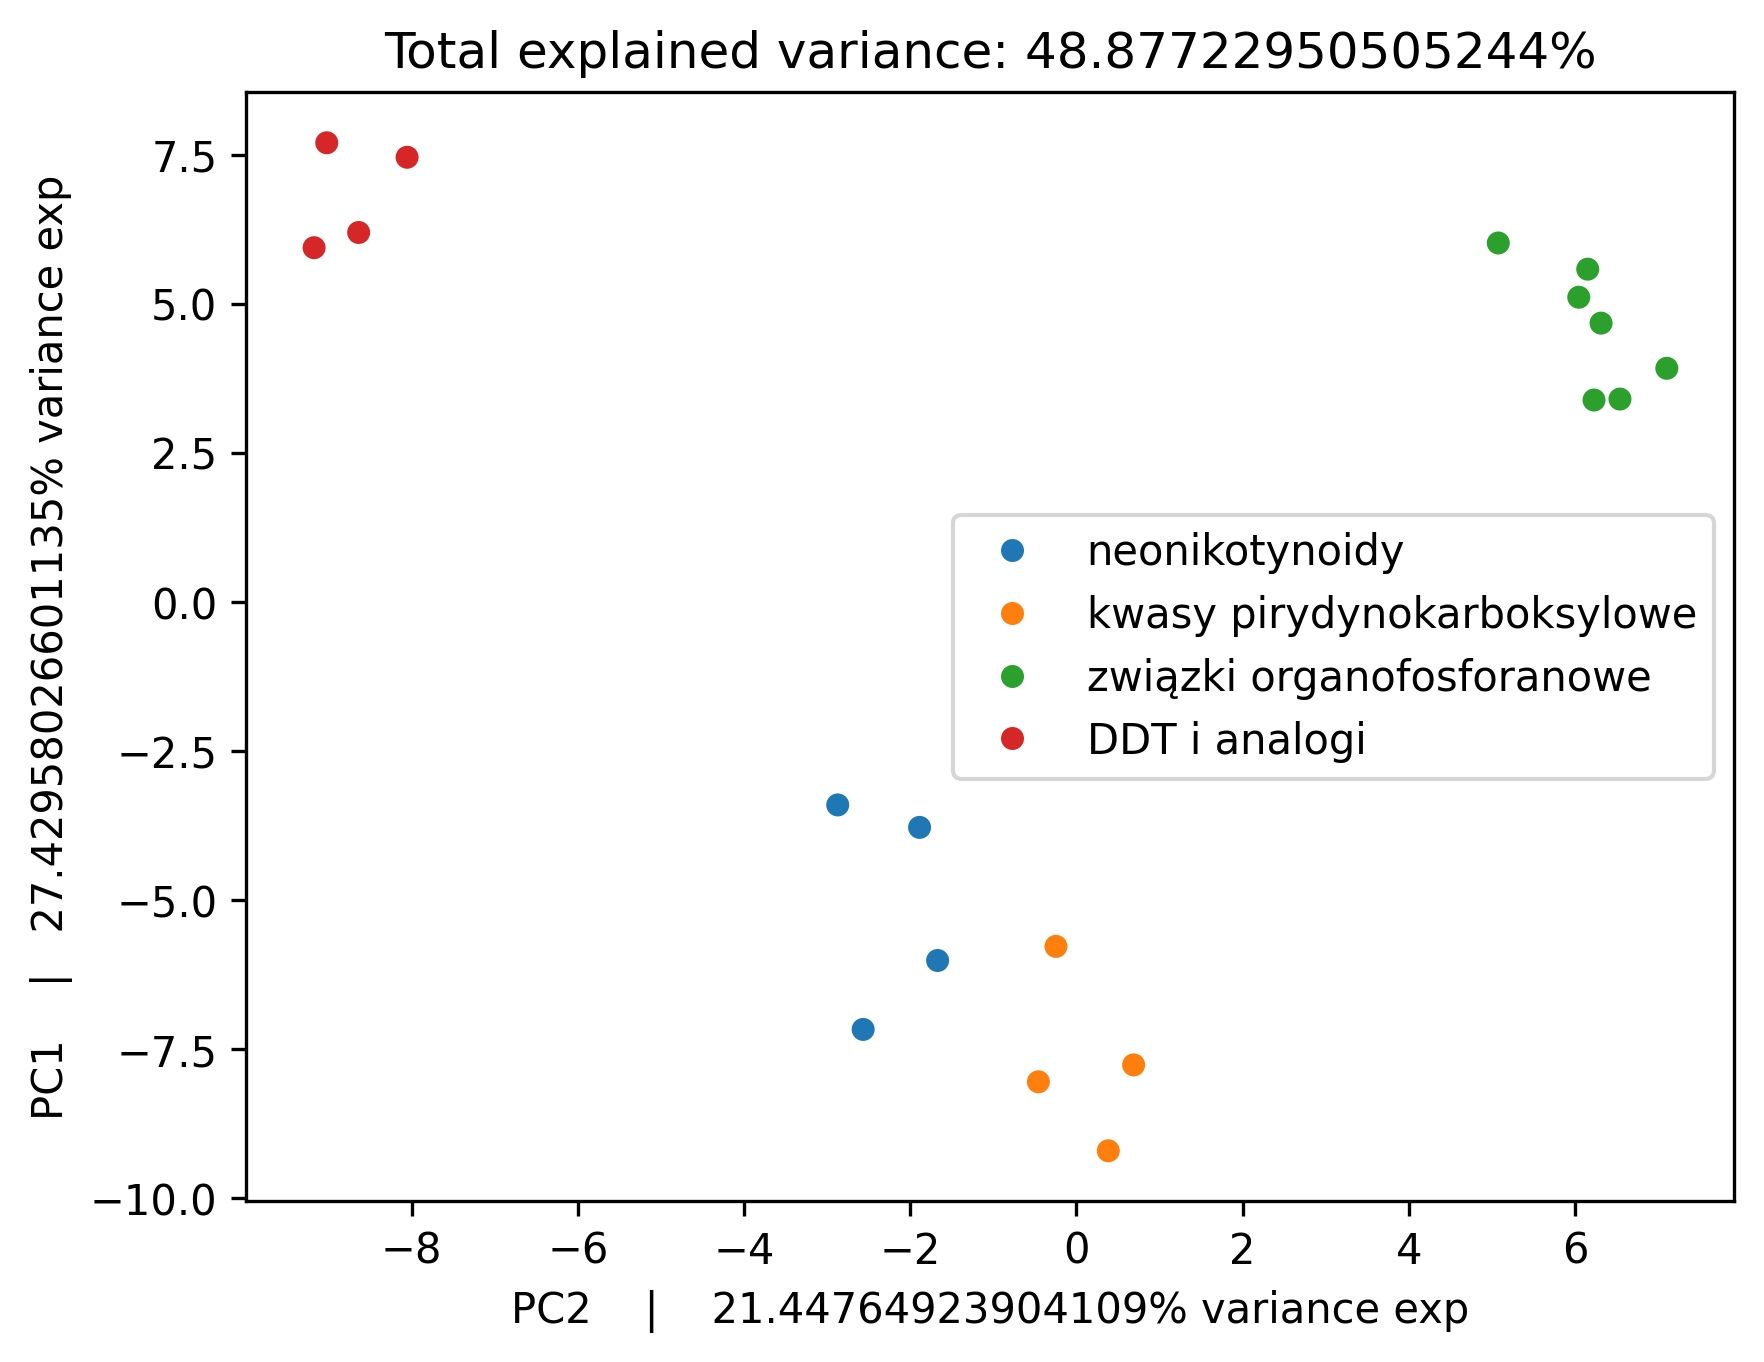
\includegraphics{21.png}
            \caption{Wykres PC2 do PC1}
        \end{figure}

    \subsection*{PC1:PC3}
        \begin{figure}[H]
            \centering
            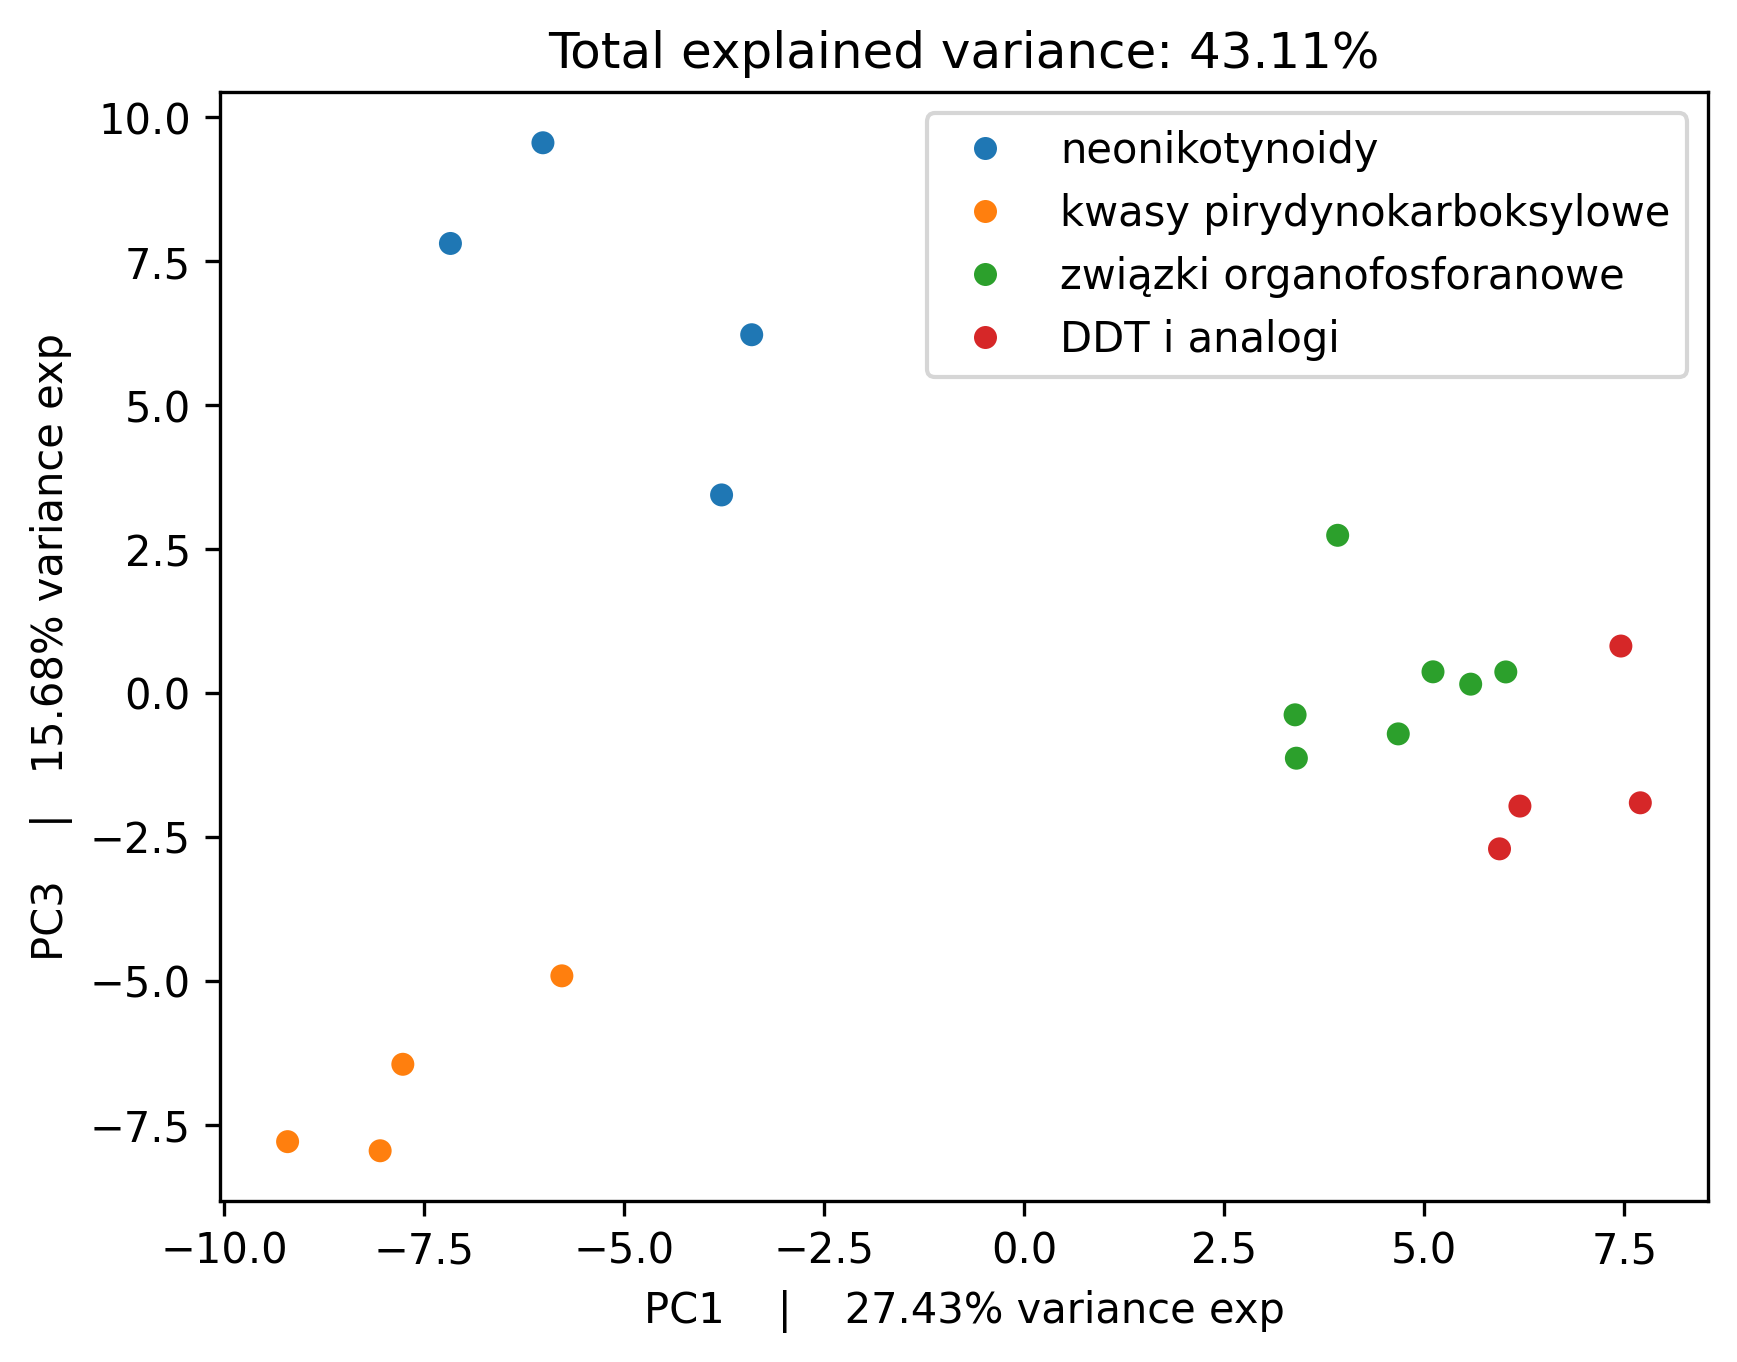
\includegraphics{13.png}
            \caption{Wykres PC1 do PC3}
        \end{figure}

    \subsection*{PC3:PC1}
        \begin{figure}[H]
            \centering
            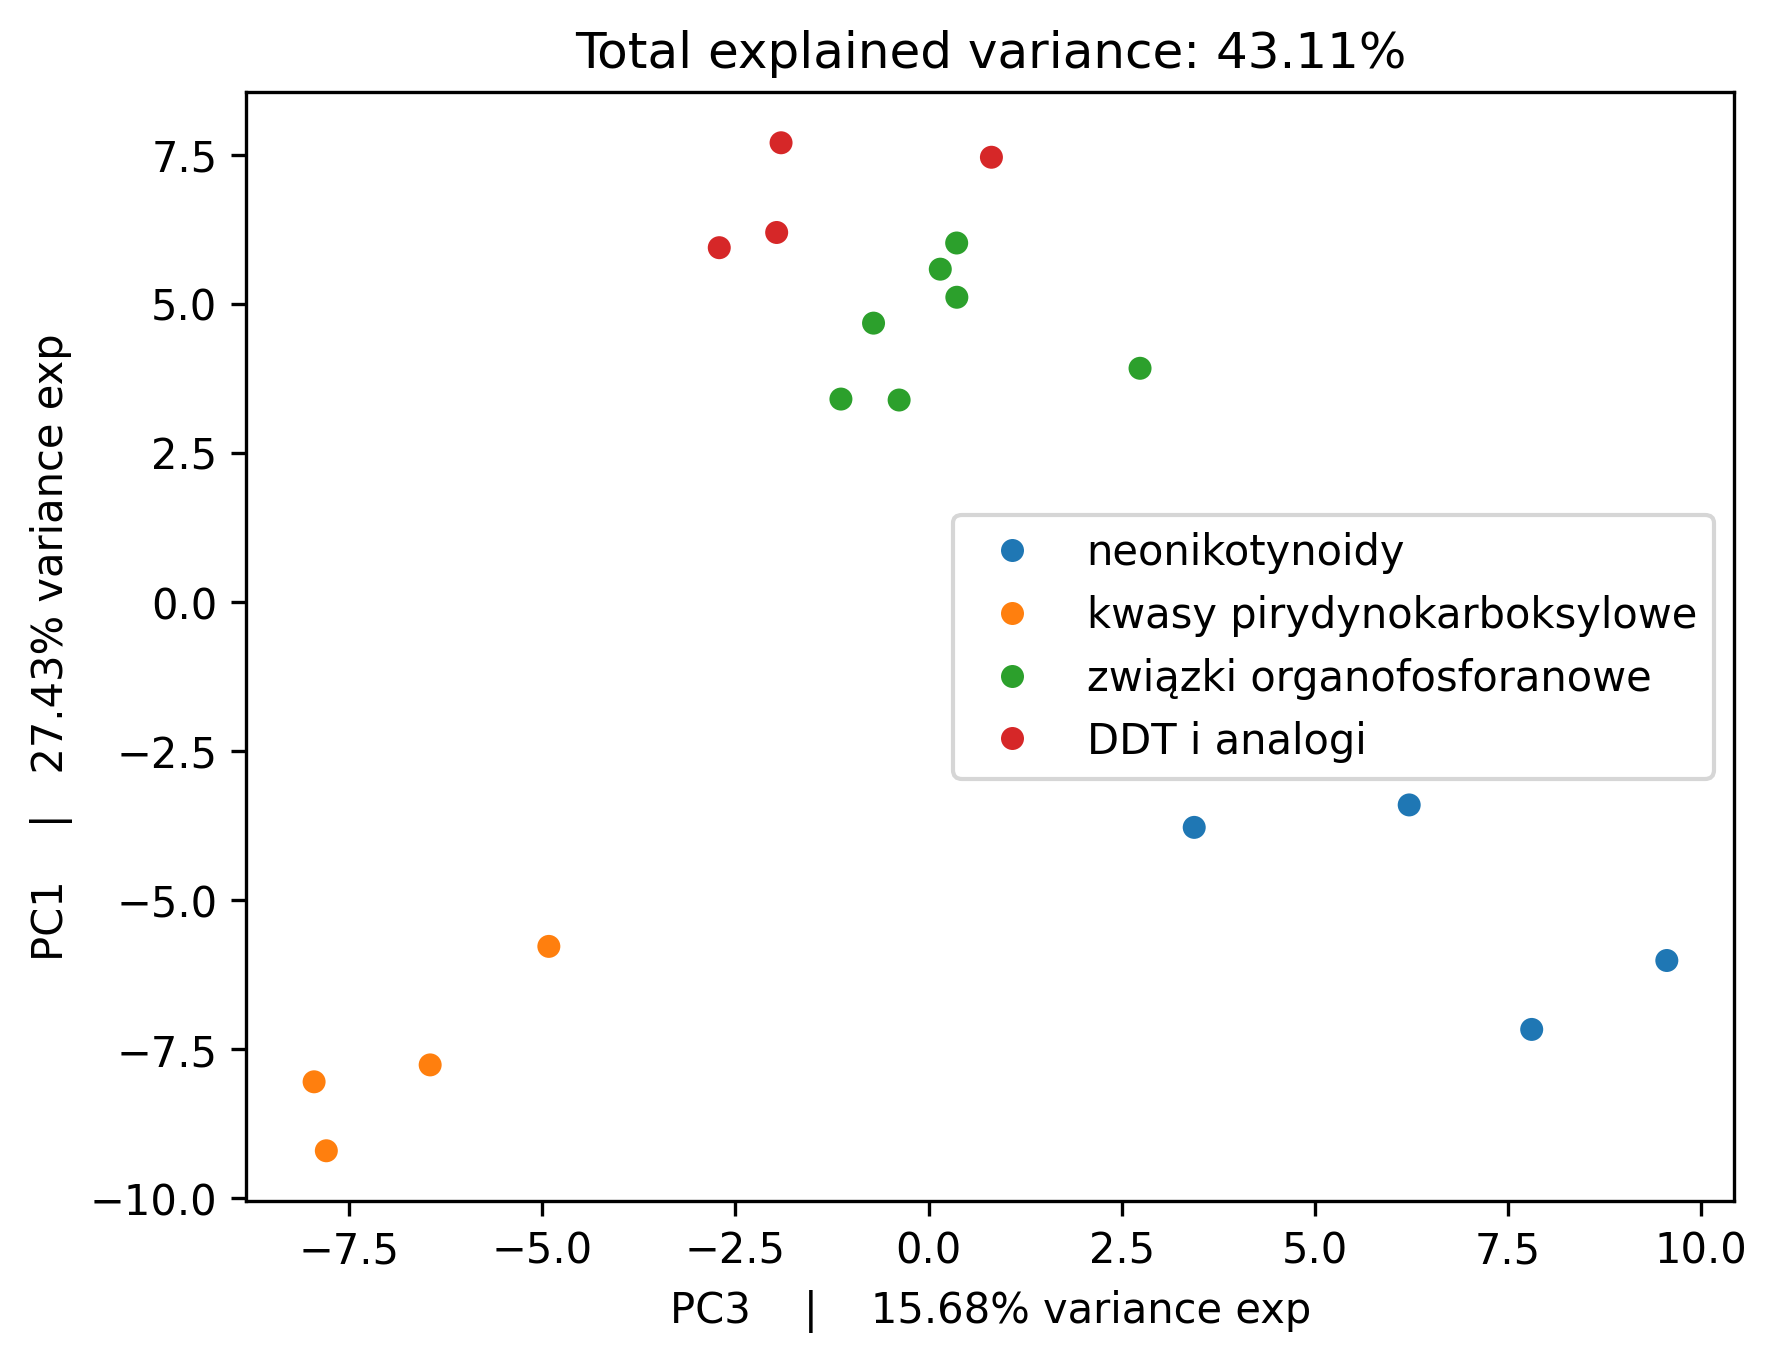
\includegraphics{31.png}
            \caption{Wykres PC3 do PC1}
        \end{figure}
    
    \subsection*{PC2:PC3}
        \begin{figure}[H]
            \centering
            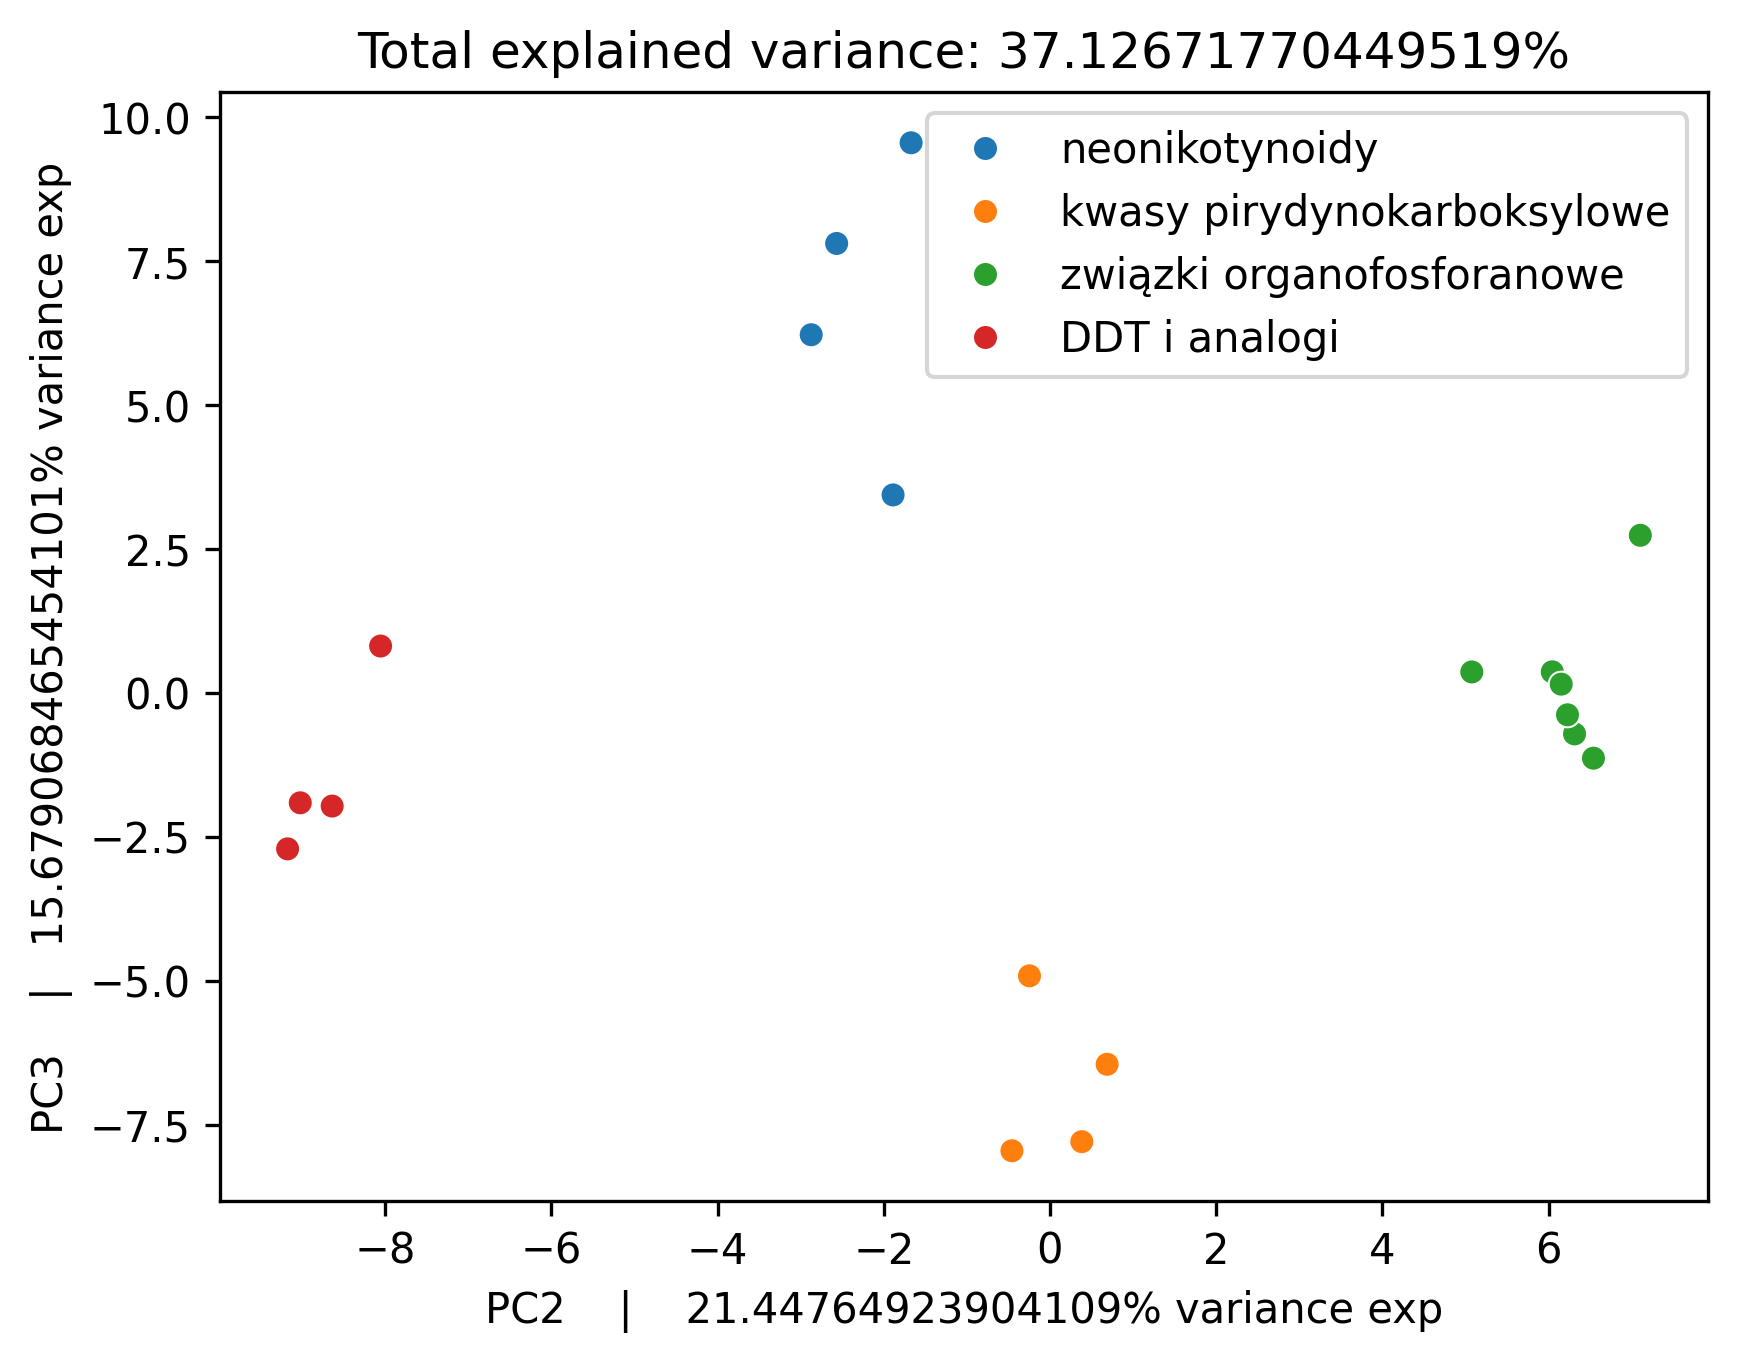
\includegraphics{23.png}
            \caption{Wykres PC2 do PC3}
        \end{figure}

    \subsection*{PC3:PC2}
        \begin{figure}[H]
            \centering
            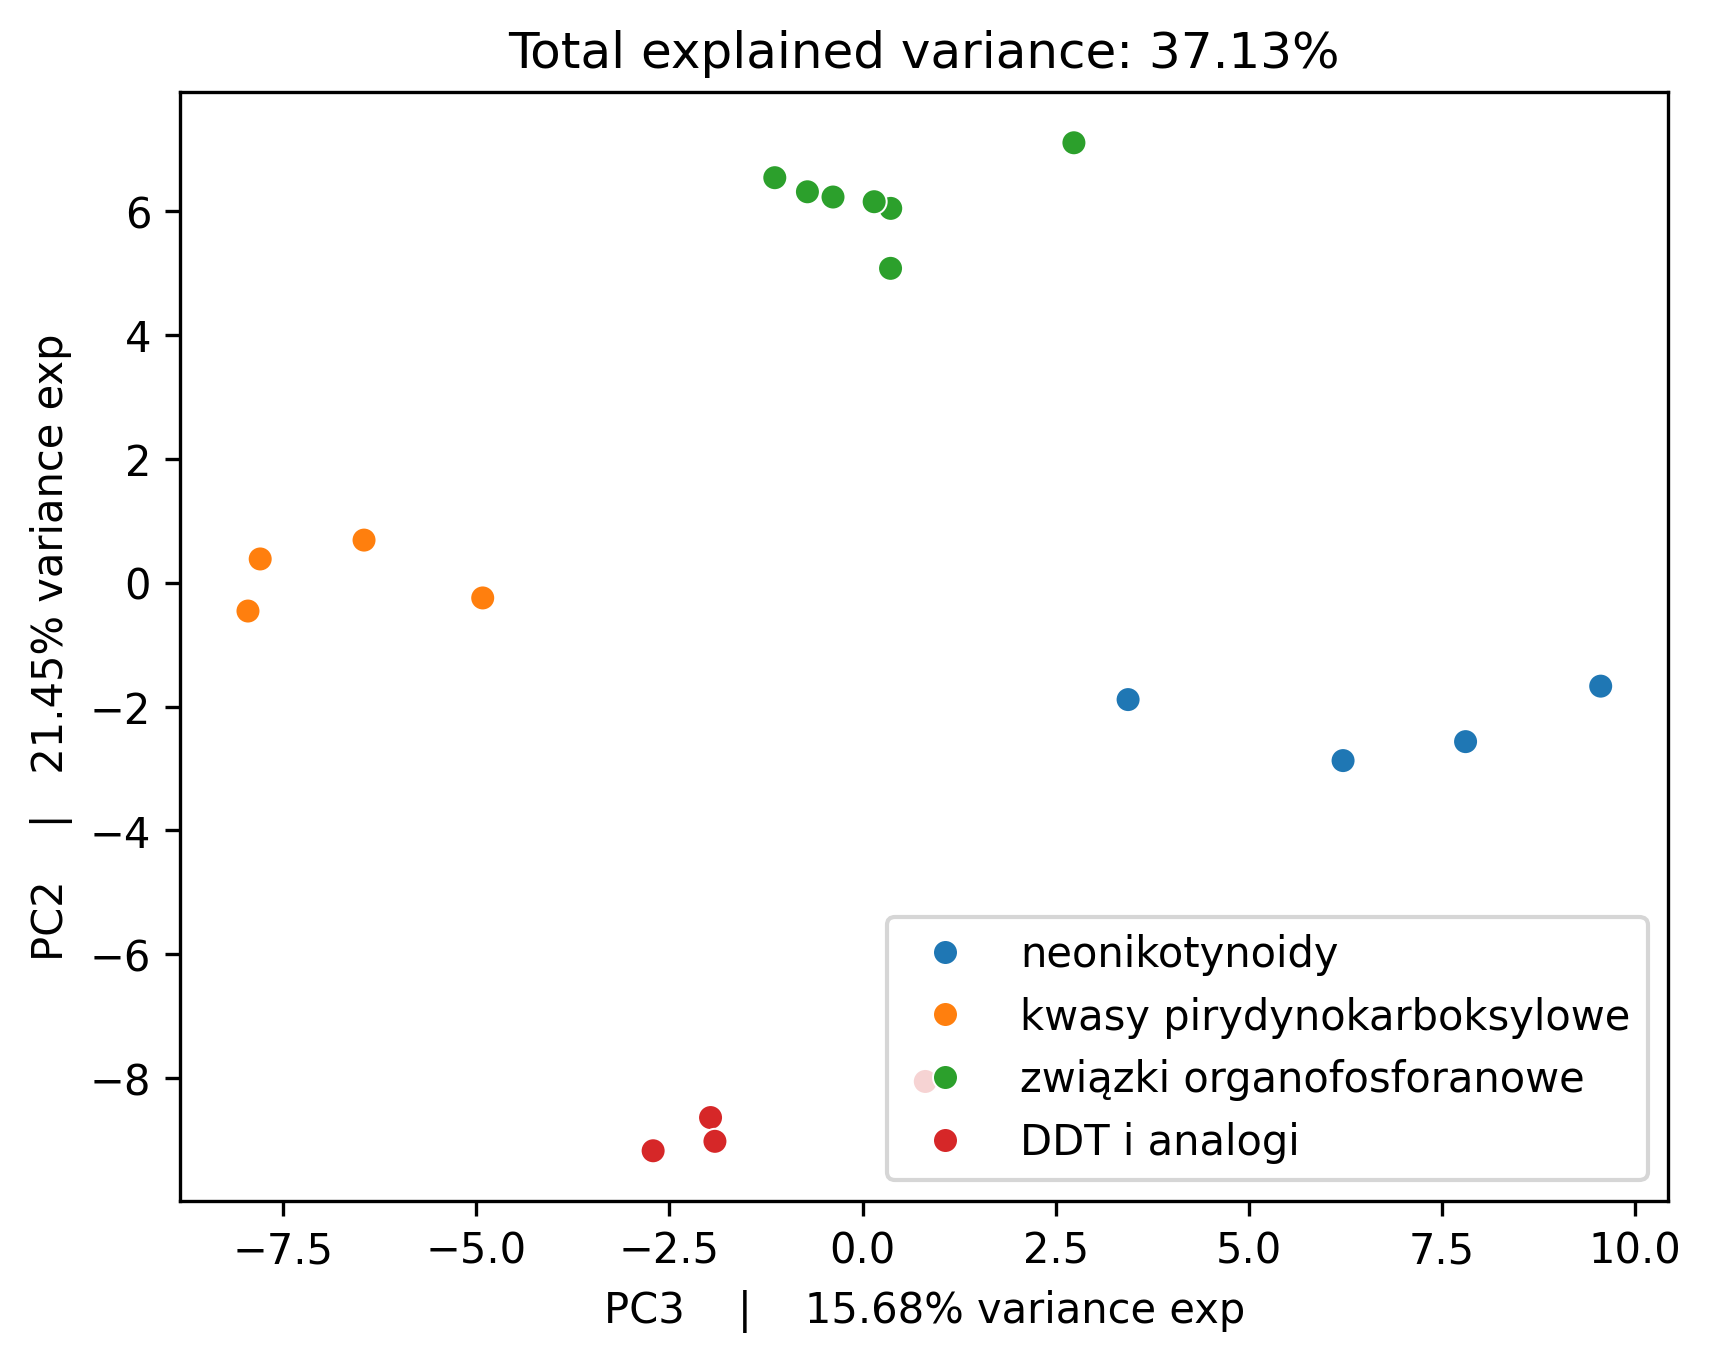
\includegraphics{32.png}
            \caption{Wykres PC3 do PC2}
        \end{figure}

\section{Obserwacje}
    
    Jak można zauważyć, powstałe wykresy oddzielają nam 4 grupy pestycydów od siebie
    w sposób bardzo czytelny. W większości przypadków są one skumulowane oraz oddzielone od siebie. Jest to
    widoczne najlepiej na zestawieniu PC2 oraz PC3. Warto zaznaczyć, że dzieje się tak pomimo najniższej sumy opisywanej wariancji.

\section{Dyskusja i wnioski}

    Spośród 4 grup, które zostały włączone do PCA tzn. (neonikotynoidy, kwasy pirydynokarboksylowe, związki organofosforowe, DDT i analogi)
    wszystkie są w podobnej odległości od siebie, dlatego ciężko byłoby stwierdzić, które się od siebie najbardziej różnią.

    Zgrupowania są raczej zwarte, oprócz neonikotynoidów, które wizualnie wykazują się najluźniejszą strukturą.

    PCA jest bardzo użyteczną techniką używaną w procesie analizy danych. Może ona służyć zarówno w celu przystępniejszego
    wyświetlenia danych, jak i jako dane wejściowe do algorytmów uczenia maszynowego. Oprócz tego metoda
    PCA może być wykorzystywana do odszumiania zdjęć, co jest według mnie bardzo interesujące. 

    W tym przypadku znana jest przynależność poszczególnych związków do grup, dlatego można było je zaznaczyć na wykresach.
    Jednak jeśli to nie byłoby wiadome, możnaby połączyć metodę PCA z metodą grupowania np. KMeans. 

    \begin{figure}
        \centering
        \subfloat[\centering grupowanie oryginalne]{{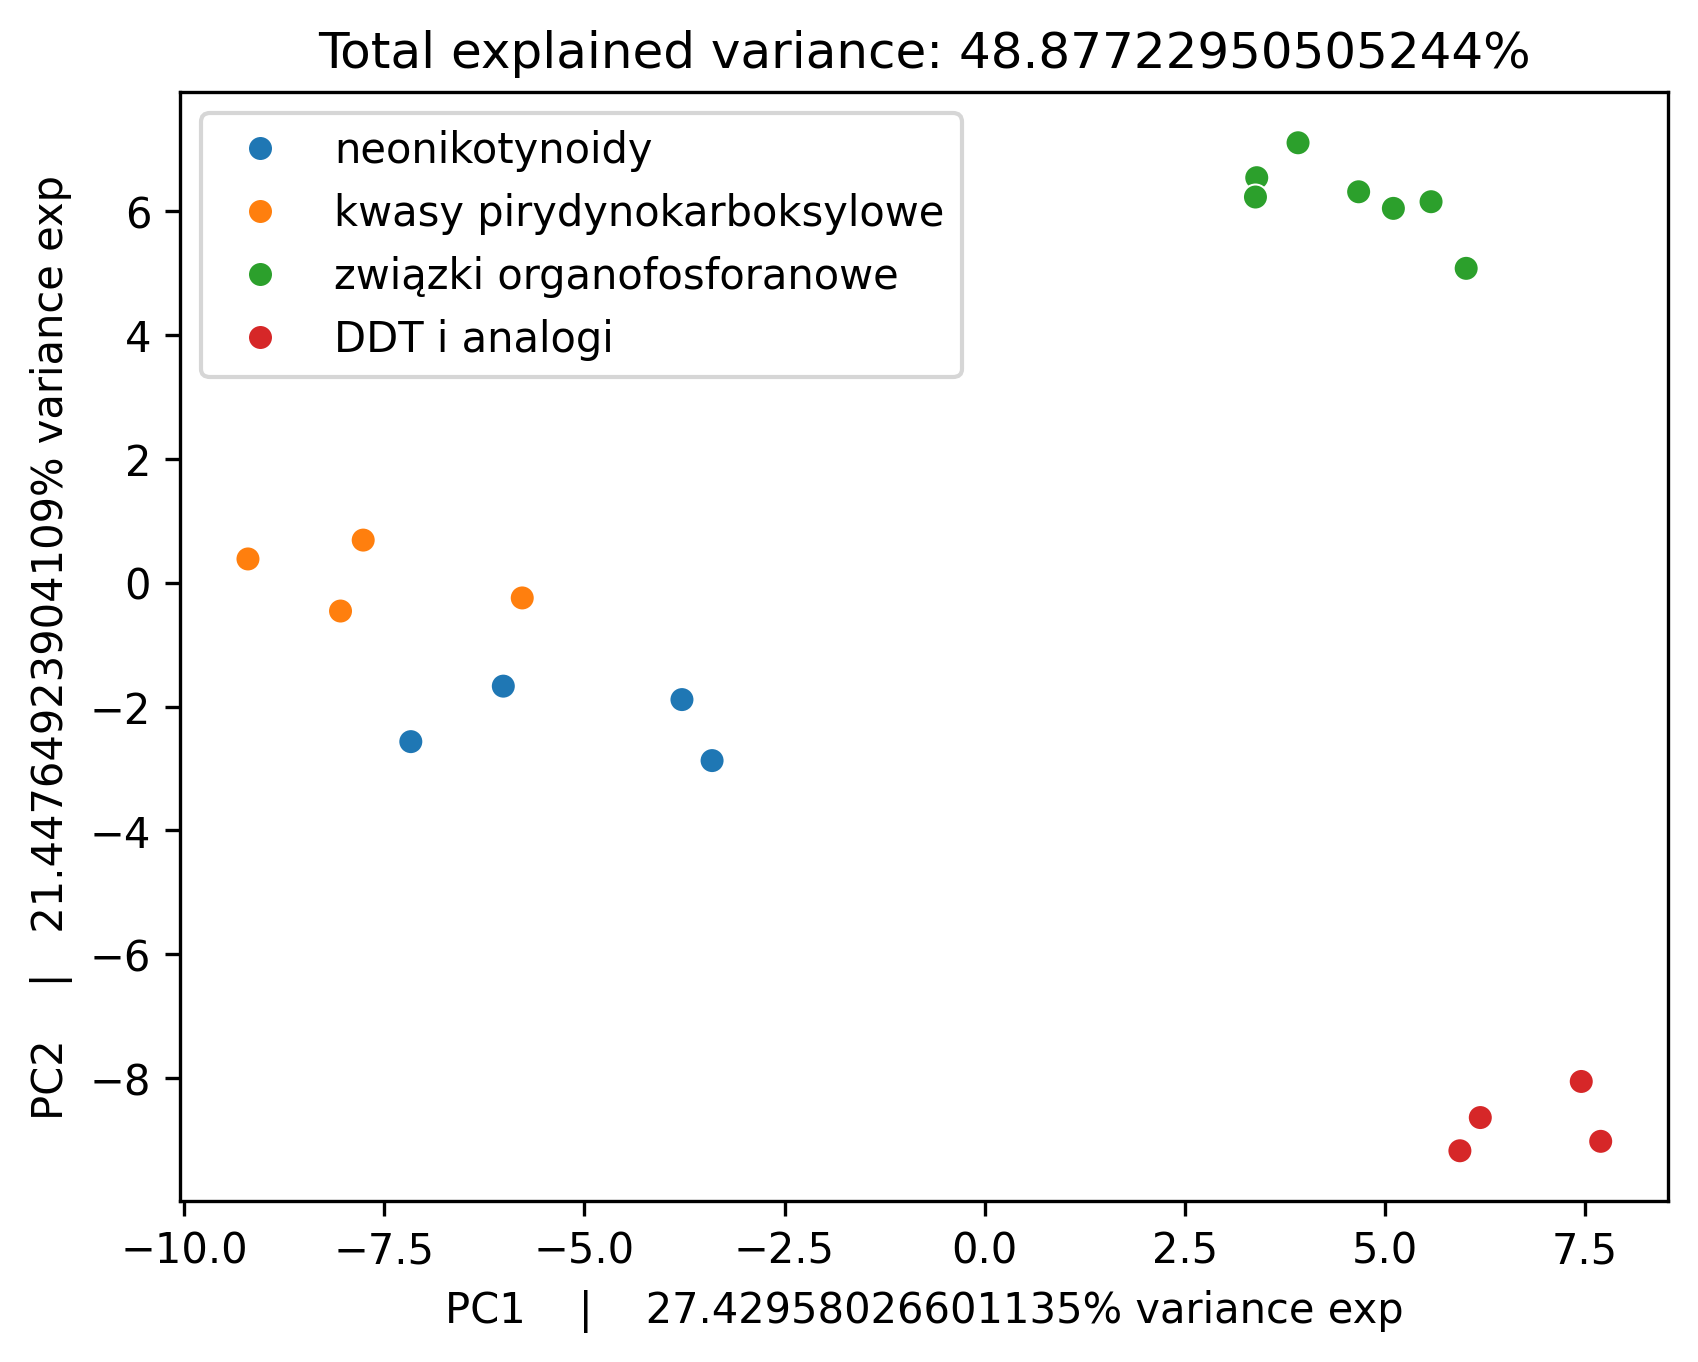
\includegraphics[width=8cm]{12.png}}}
        \qquad
        \subfloat[\centering grupowanie KMeans]{{\includegraphics[width=8cm]{12\_kmeans.png}}}
        \caption{Zestawienie wykresów względem różnego grupowania}
    \end{figure}

    Muszę przyznać, że na wykresie z grupowaniem KMeans jest jedna wartość więcej, niż powinna być.
    Po analizie kodu muszę przyznać, że nie wiem, skąd ten błąd się wziął. Jeśli przymknąć na niego oko,
    otrzymamy dokładnie takie samo grupowanie.

\end{document}